\subsection{Opciones del lector}

El lector cuenta con una pequeña \emph{pantalla TFT} y unos pocos botones para su manejo. La primera opción que se da al lector es su vinculación con la cuenta del usuario y para ello se muestra el siguiente aviso en la \emph{pantalla TFT}:

\begin{figure}[h!]
    \centering
    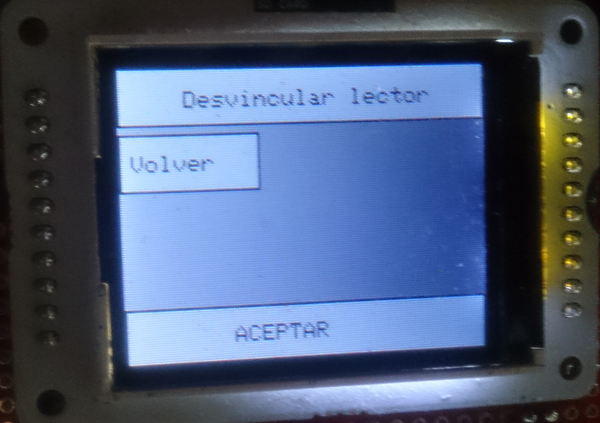
\includegraphics[keepaspectratio,width=0.6\textwidth]{lector_desvincular.png}
    \caption{Vinculando lector}\label{fig:lector_desvincular}
\end{figure}

Una vez se ha vinculado, escaneando para ello los dos códigos de barras generados por la aplicación web, se muestra la siguiente pantalla con las opciones disponibles:

\begin{figure}[h!]
    \centering
    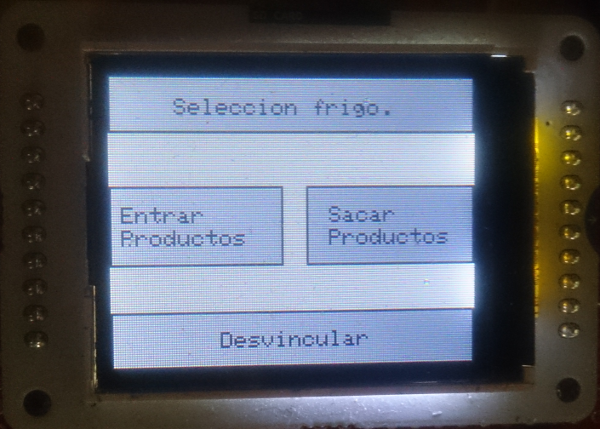
\includegraphics[keepaspectratio,width=0.6\textwidth]{lector_home.png}
    \caption{Pantalla de inicio del lector}\label{fig:lector_home}
\end{figure}

Para acceder a cada opción de menú hay que pulsar cada botón correspondiente; superior para listar los frigoríficos, inferior para desvincular el producto, y laterales para añadir o o quitar productos del frigorífico.

Al acceder a cada opción de menú se muestra una pantalla diferente, con una opción para \emph{Volver} y opcionalmente alguna otra u otras opciones:

\begin{itemize}

    \item Selección del frigorífico activo

        Esta opción de menú nos permitirá elegir el frigorífico sobre el que se realizarán las acciones (entrada / salida) de productos.

        \begin{figure}[h!]
            \centering
            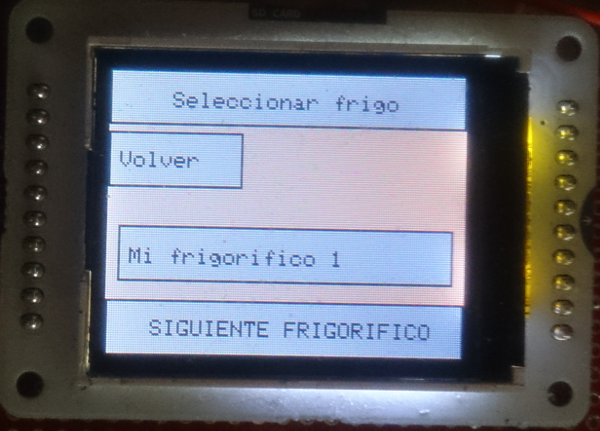
\includegraphics[keepaspectratio,width=0.6\textwidth]{lector_seleccion_frigo.png}
            \caption{Selector de frigoríficos}\label{fig:lector_seleccion_frigo}
        \end{figure}


        A través del botón inferior podemos ir moviéndonos entre los frigoríficos que dispone el usuario, para ello se han traído a través de una petición \emph{RESTful}. Una vez nos encontramos sobre el frigorífico que queremos dejar configurado basta con pulsar en la tecla \emph{Volver}.

        En el caso de no contar con frigoríficos se muestra el siguiente mensaje en pantalla:

        \begin{figure}[h!]
            \centering
            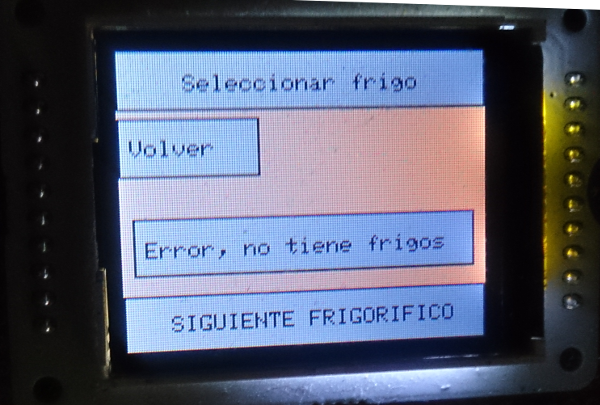
\includegraphics[keepaspectratio,width=0.6\textwidth]{lector_no_tiene_frigos.png}
            \caption{No dispone de frigoríficos}\label{fig:lector_no_tiene_frigos}
        \end{figure}

    \item Modo entrada de productos

        Para introducir productos al frigorífico seleccionamos la opción de menú para \emph{Añadir productos al carrito}, donde se activará la lectura de productos por \emph{código de barras} ó a través del \emph{lector RFID}. En la pantalla se muestra la siguiente información:

        \begin{figure}[h!]
            \centering
            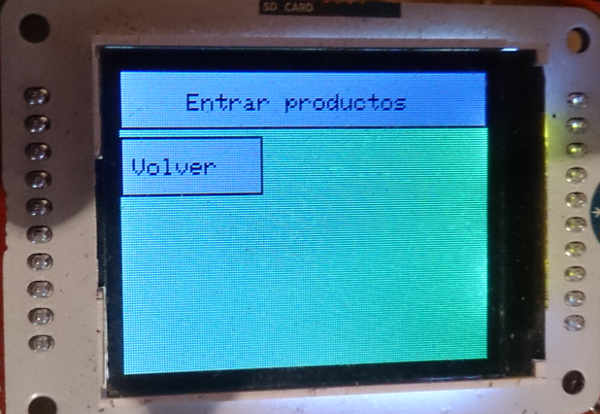
\includegraphics[keepaspectratio,width=0.6\textwidth]{lector_entrar_productos.png}
            \caption{Entrar productos en el frigorífico}\label{fig:lector_entrar_productos}
        \end{figure}

        Al escanear un producto se realiza la petición \emph{RESTful} para añadirse al frigorífico activo.

        Al pulsar el botón izquierdo se regresa a la pantalla anterior para acceder a las opciones de menú.

    \item Modo salida de productos

        Para sacar productos del frigorífico nos colocaremos en esta opción del menú el cual activará la lectura de productos por \emph{código de barras} ó a través del \emph{lector RFID}.

        \begin{figure}[h!]
            \centering
            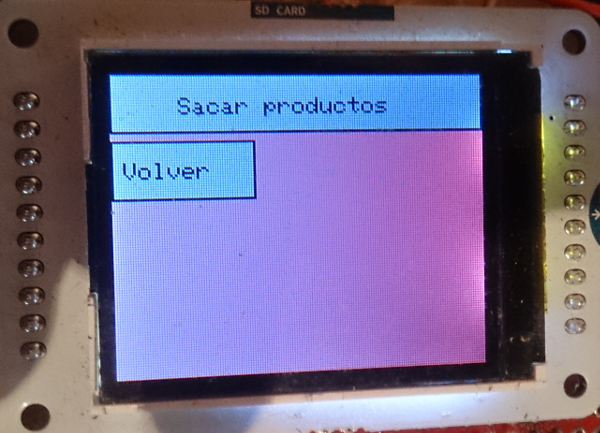
\includegraphics[keepaspectratio,width=0.6\textwidth]{lector_sacar_productos.png}
            \caption{Sacar productos del frigorífico}\label{fig:lector_sacar_productos}
        \end{figure}

        Al pulsar el botón izquierdo se regresa a la pantalla anterior para acceder a las opciones de menú.

    \item Desvinculación del aparato

        Esta opción de menú borrará de la memoria \emph{MicroSD} la clave pública de acceso, con lo cual se quedará desvinculado el lector de nuestra cuenta de usuario en la aplicación web. Además se lanza una petición \emph{RESTful} para indicar al servidor que se quiere desvincular el lector.

        Antes de iniciar la desvinculación se muestra una pantalla de confirmación al usuario, debiendo pulsar el botón inferior para \emph{Aceptar} la opción:

        \begin{figure}[h!]
            \centering
            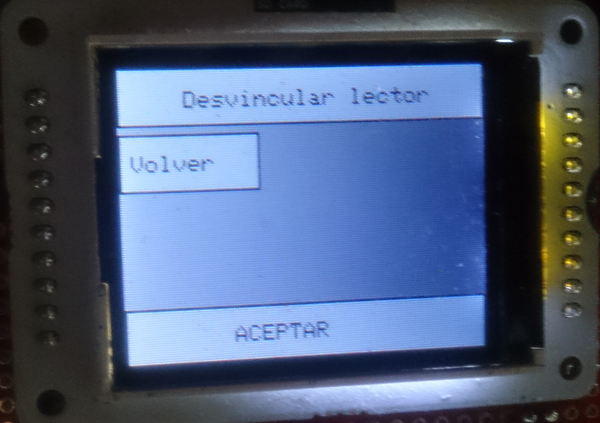
\includegraphics[keepaspectratio,width=0.6\textwidth]{lector_desvincular.png}
            \caption{Confirmar desvincular lector}\label{fig:lector_desvincular}
        \end{figure}

        Una vez se confirma, se lanza la petición al servidor y se procede a eliminar la clave pública, una vez desvinculado se muestra la pantalla para volver a iniciar la vinculación del lector:

        \begin{figure}[h!]
            \centering
            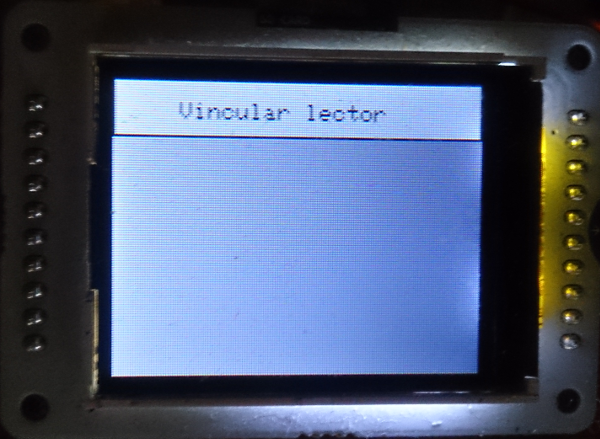
\includegraphics[keepaspectratio,width=0.6\textwidth]{lector_vincular_lector.png}
            \caption{Vincular lector}\label{fig:lector_vincular_lector}
        \end{figure}

\end{itemize}